\documentclass[a4paper, 12pt]{article}

\usepackage{graphicx}
\graphicspath{{./images/}}
\usepackage{float}
\usepackage{wrapfig}
\usepackage{blindtext}
\usepackage{amsmath}
\usepackage{amssymb}
\usepackage{fancyhdr}
\usepackage[margin=0.9in]{geometry}
\usepackage[sorting = none]{biblatex}
\addbibresource{progress.bib}
\usepackage[colorlinks=true,linkcolor=red, citecolor=black, urlcolor = black]{hyperref}%
\usepackage{appendix}
\usepackage{pythonhighlight}
\usepackage{subcaption}

\begin{document}

\title{\textbf{GW Burst Progress Documentation}}
\author{Ethan Millar}
\date{}
\maketitle

\section{Adding Noise}

\begin{figure}[H]
  \centering
  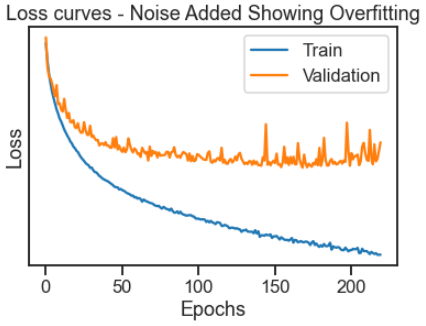
\includegraphics[scale = 0.7]{Overfit.PNG}
  \caption{Loss curves comparing training and validation set demonstrating overfitting in the model}
  \label{fig:overfit}
\end{figure}

Steps relating to the model were taken to try and optimise the model, first attempt was with regularisation, in particular altering the weight decay parameter in the adam optimiser from $1 \times 10^{-6}$ to $  \times 10^{-4}$.

I ran the first 50 epochs to compare to the initial overfitted curves

\begin{figure}[H]
\begin{subfigure}{.5\textwidth}
    \centering
    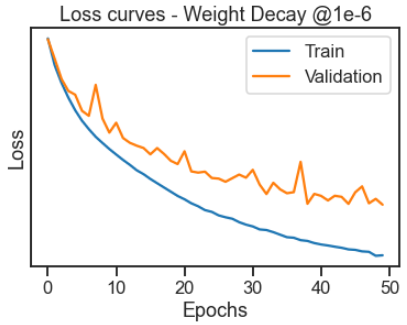
\includegraphics[width=1\textwidth, scale = 0.5]{Weightdecay0.PNG}
    \caption{Loss curves after increasing the weight decay to $1 \times 10^{-6}$}
    \label{fig:wd0}
\end{subfigure} \hfill
\begin{subfigure}{.4\textwidth}
    \centering
    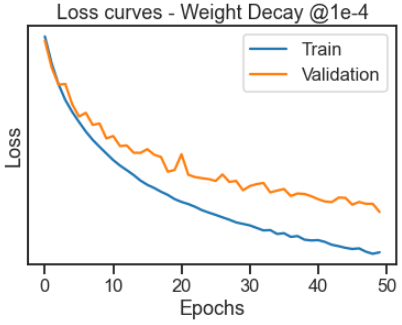
\includegraphics[width=1.1\textwidth, scale = 0.5]{Weightdecay1.PNG}
    \caption{Loss curves after increasing the weight decay to $1 \times 10^{-4}$}
    \label{fig:wd1}
\end{subfigure} \hfill
\begin{subfigure}{.4\textwidth}
    \centering
    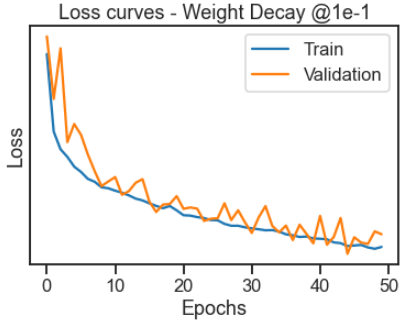
\includegraphics[width=1.1\textwidth, scale = 0.5]{Weightdecay2.PNG}
    \caption{Loss curves after increasing the weight decay to $1 \times 10^{-1}$}
    \label{fig:wd2}
\end{subfigure}%
\centering
\caption{Comparing Loss Curves when altering weight decay}

\end{figure}

\begin{figure}[H]
  \centering
  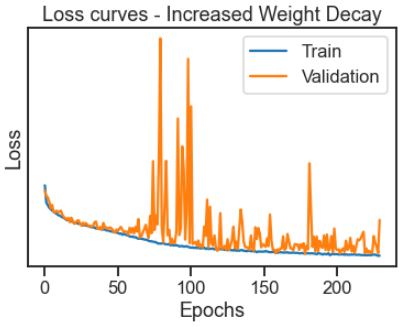
\includegraphics[scale = 0.8]{LossSpikes.PNG}
  \caption{Running for 225 epochs with the weight decay increased to $1 \times 10^{-1}$}
  \label{}
\end{figure}

Next approach is to decrease the learning rate from $1 \times 10^{-3}$ to $1 \times 10^{-4}$

\end{document}
